\chapter{Троя даже на Борщаге}

Доминиканский монах Мартин Груневег (отец Венцеслав), духовник Марины Мнишек, оставил в своих записках\cite{gruneveg} сведения о Киеве, где был проездом в 1584 году. По его словам, русские верят, будто Троя находилась на месте Киева. В скобках дается написание названий как в подлиннике:

\begin{quotation}
16 Октября кормили лошадей в Брусилове\footnote{Брусилов на реке Здвиж есть и поныне, тогда же это было местечко на торговом пути из Житомира в Киеве. Брусилов управлялся по магдебургскому праву. А другой Брусилов, около Чернигова, принадлежал Адаму Киселю.}, 5 миль от Корестишова. Лежит в лесу на реке, окружен деревянными крестовинами. Это пустой городок, около Рынка замок, а в середине рынка церковь. Ночевали в лесу.

17 Октября мимо высокого круглого проехали вала, стоящего в глухом лесу с небольшим полем вокруг, окружен вдали рвом. Жители называют его Лось (Los). Я прошел кругом по верху вала. Кормили лошадей в лесу, переехали через реку Роман (Roman fl.) ночевали в лесу у реки Борщаговки (Boersgofka fl.), 8 1/2 мили\footnote{Здесь и далее Груневег пользуется немецкими милями. Немецкая миля равна 7420 метра. 8,5 немецкие мили = 63,07 километра.} от Брусилова.

Русские, поскольку они слышали, каким могущественным был город Киев, что он был столицей их Князей, что его часто упоминают летописи в связи с его войнами и другими важными событиями, что еще сегодня видны драгоценные творения церкви Софии, как и простирающиеся на несколько миль разрушенные сооружения, говорят, что Город занимал 7 немецких миль\footnote{51,91 км.} в ширину, а многие из них верят, будто Троя находилась на этом месте\footnote{Die Reussen, die weile sie hören wie eine mechtige statt Kiof was, das sie ist gewesen der sietz ihrer Fuersten, das sie die kronik wegen ihres krieges unde wichtiger geschiente öfters gedencket, das man noch heutte das köstliche werkder kierche Zophie vor äugen hatt, auche etliche meilen umher tzerstört gemewrs siet, sprechen sie, die Statt sey sieben teutzer meilen weit gewesen, gleuben auch ihrer fiele, es sey Troya am selben ortte standen.}.

И они поэтому говорят, что этой реке дали такое имя потому, что там находился Барсч рынок, прямо на том месте, где мы расположились\footnote{Und derhalb sprechen sie, man habe diesem wasser dofonn solchen namen geben, das dabey derr Barßcz markt was, und an dem orte, dawir lagen.}. Киев, я думаю, был довольно большим городом, но [считая] отнюдь не в русских милях, а одна немецкая миля, взятая в квадрат, составляет большой город, Данциг вряд ли имеет [такие размеры], и я считаю,что вряд ли он был больше, чем теперешний Данциг в целом. Это могло быть, несмотря на то, что данное место находится далеко от города, но оно могло быть названо борщевым рынком или местом, даже если в те времена борщ не поступал в продажу. К тому же Русские покупают борщ редко или никогда, потому что каждый готовит его сам у себя дома, поскольку это их повседневная еда и питье.

Если бы за борщом на 1 пфенниг нужно было бы нестись за несколько миль, он, скорее, стоил бы, как вино. Поэтому это грубое заблуждение (но не удивительное) грубого народа, будто Киев по площади занимал 7 миль, что борщ нигде не продавался, кроме как в этом месте, удаленном от Киева на 1 1/2 мили\footnote{То есть 11,13 км. от Подола. Груневег называет нынешний Подол Киевом. Предположу, что речь идет о Петропавловской Борщаговке или Софиевской Борщаговке.}. Кроме того, известно, что Троя находится в Малой Азии едва ли не в трехстах милях от Киева.
\end{quotation}

Оставим шутки Груневега про борщ в стороне, оголим записки до сути. Перебравшись через реку Роман (возможно, Репин-Ирпень), монах заночевал в лесу у реки Борщаговки (теперь ее иногда называют Нивкой), где узнал, что тут, прямо на этом месте, был Борщевой рынок, и по нему названа река. И раньше, мол, Город занимал 51 километр в ширину, и это была легендарная Троя.

\begin{center}
\includegraphics[width=\textwidth]{chast-troya/troya-kiev/\myimgprefix IMG_3976.JPG}

\textit{2014 год, речка Борщаговка.}
\end{center}

\newpage
\begin{center}
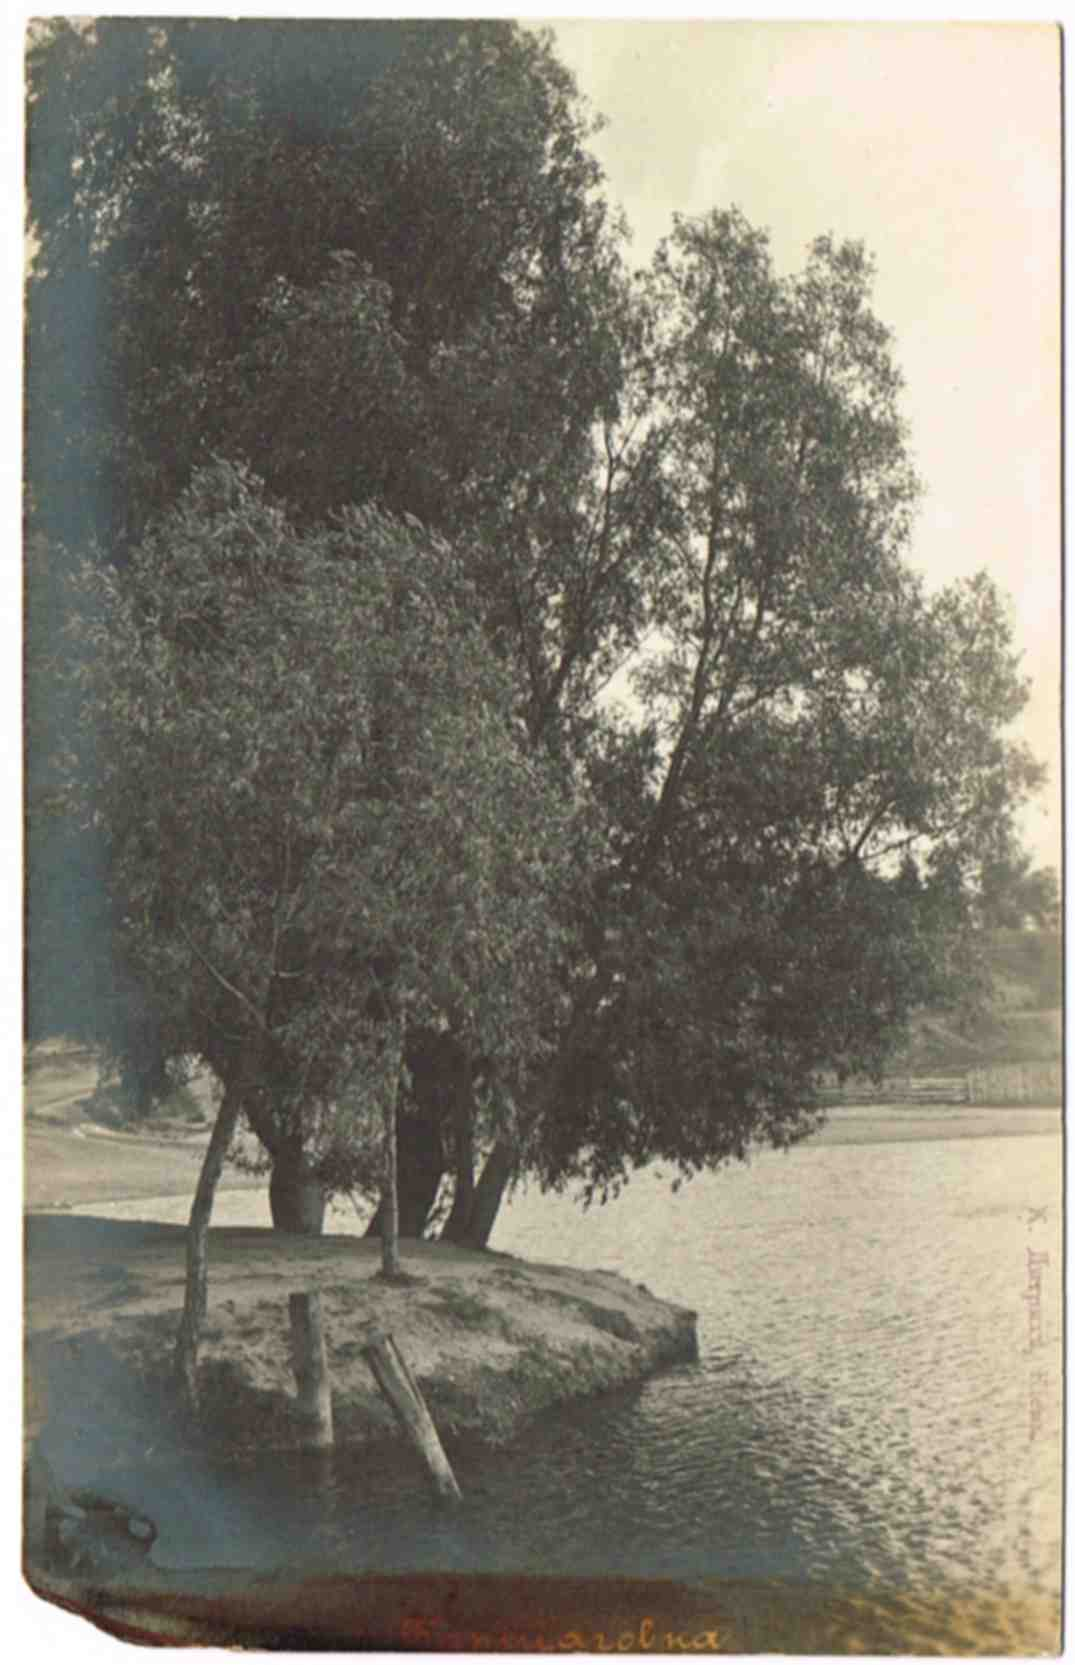
\includegraphics[width=\textwidth]{chast-troya/troya-kiev/borsh.jpg}

\textit{Борщаговка, дореволюционный снимок.}
\end{center}
\newpage

Конечно, не могло быть рынка, где торговали одним только борщом. 

Речка Борщаговка, как и одноименная местность, в земельных документах 16-17 веков именуется Борщовкой. Разберем это слово. Буква «щ» могла произноситься как «ч», разница невелика. На берегу Днепра мы знаем местность Боричев, он же Боричов. Нетрудно переделать в Боричовку или Борщовку. Я не отождествляю Боричев и Борщовку, я ищу подобия.

Со стороны Днепра был, упрощенно говоря, таможенный пункт – Боричов. В слове «борич» заключено значение побора, налога, взимаемого с купцов. Так почему в 11 километрах от летописного Боричева не могло быть другого таможенного пункта, с базаром при нем? Боричов рынок! Борщов рынок!

Река Борщовка – приток Ирпеня (в старину Репина). На Борщовке невесть с каких пор были пруды, хотя вероятно она могла быть широкой и по естественным причинам. Направление течения у Борщовки противоположно Лыбеди.

А на берегу реки Ирпень стояла знаменитая крепость Белгородка, ныне поселок к западу от Софиевской Борщаговки, издавна обжитое место. Сей Белгород был достаточно велик, в некие давние времена даже сопоставим с тогдашним же Черниговом, и находился на торговом пути из Киева к западу – в Галицию.

Конечно же, сам бог велел на дороге, водной и сухопутной, между Белгородкой и Киевом, соорудить облагаемый поборами в пользу Киева, Боричов рынок! Боричов торг.

И слово «торг» выплывает в другом источнике.

Михалон Литвин в трактате «О нравах татар, литовцев и москвитян»\cite{litvin}, впервые изданном в 1615 году на латинском языке, кроме прочего рассказывая о Киеве, говорит такое:

\begin{quotation}
Так считается, что и Илион (Ilium), или Троя (Troiam), некогда находились на киевской территории (territorio Kioviensi), в плодороднейших степях и живописнейших лесах. Здесь можно видеть памятники, от которых ныне сохранились развалины, подземелья, гроты, мраморные плиты и остатки мощных стен. Это давно покинутое, но весьма удобное для обитания место называется ныне Торговица (Torgovitza).
\end{quotation}

Я не помещаю в своей книге все средневековые источники, где Киев связывается с Троей либо такая связь опровергается. Главное, что такое мнение бытовало, оно просочилось в записки путешественников и в литературные произведения – например, в поэму «Роксолания» (1584) Себастиана Кленовича, в «Днепровские камены» (1620) Ивана Домбровского.
